\documentclass[11pt,a4paper]{article}
\usepackage[T1]{fontenc}
\usepackage{lmodern}
\usepackage[margin=2.5cm]{geometry}
\usepackage{algorithm,algpseudocode,caption,hyperref}
% ---- shared preamble material (included by paper.tex and report.tex) ----
\usepackage{amsmath,amssymb,booktabs,siunitx,xcolor,multirow,graphicx}
\usepackage{pgfplots,pgfplotstable}
\usepackage{tikz}
\usetikzlibrary{positioning,arrows.meta,fit,calc}
\pgfplotsset{compat=1.16}
\newif\ifillustrative \illustrativefalse  % data/*.csv are generated by sim/analyze.py from results/
% Generated by sim/analyze.py. Do not edit.
\newcommand{\hOneAdaptSlope}{0.628} % results/burst.jsonl (fit)
\newcommand{\hOneCapSlope}{0.00232} % results/burst.jsonl (fit)
\newcommand{\hOneFpSlope}{5.92} % results/burst.jsonl (fit)
\newcommand{\hOneRrSlope}{6} % results/burst.jsonl (fit)
\newcommand{\kneeFps}{92.1} % results/fps.jsonl (drop rate crosses 1%)
\newcommand{\kneePredFps}{160} % results/predictions.json
\newcommand{\policyFps}{120} % results/policy.jsonl
\newcommand{\predCAPBound}{0.72} % results/burst.jsonl, predictions.json
\newcommand{\predCAPMax}{2.39} % results/burst.jsonl, predictions.json
\newcommand{\predCAPP99}{1.42} % results/burst.jsonl, predictions.json
\newcommand{\predFPBound}{5.2} % results/burst.jsonl, predictions.json
\newcommand{\predFPMax}{8.17} % results/burst.jsonl, predictions.json
\newcommand{\predFPP99}{7.11} % results/burst.jsonl, predictions.json
\newcommand{\predRRBound}{10.3} % results/burst.jsonl, predictions.json
\newcommand{\predRRMax}{12.1} % results/burst.jsonl, predictions.json
\newcommand{\predRRP99}{10.8} % results/burst.jsonl, predictions.json
  % every number in the text; each macro names its source
\newcommand{\tbd}[1][X]{\textcolor{red}{[#1]}}
\newcommand{\illusnote}{\ifillustrative\\[-2pt]\textcolor{red}{\scriptsize ILLUSTRATIVE SHAPE, NOT RESULTS: replace data/*.csv}\fi}
\newcommand{\imu}{\textsc{imu}}
\newcommand{\cam}{\textsc{cam}}
\newcommand{\npu}{\textsc{npu}}
\newcommand{\pone}{\ensuremath{p_{99}}}
\pgfplotsset{dmaplot/.style={width=\linewidth,height=0.72\linewidth,grid=major,
  grid style={gray!25},tick label style={font=\scriptsize},label style={font=\footnotesize},
  legend style={font=\tiny,at={(0.02,0.98)},anchor=north west},every axis plot/.append style={thick,mark size=1.6pt}}}

\pgfplotsset{dmaplot/.append style={width=0.8\linewidth}}
\title{DMA-Sense: Bus Contention, Burst Sizing and Frame-Drop Trade-offs\\on a Drone SoC\\[2pt]\large Project Report}
\author{Ahad Ulla Baig \and Divisha Gera \and Charithra G\\Dept. of Artificial Intelligence and Machine Learning, Ramaiah Institute of Technology, Bengaluru, India}
\date{\today}
\begin{document}
\maketitle
\begin{abstract}
\noindent This report documents the design, simulator, traces and experiments of DMA-Sense, a study of whether smart bus and DMA scheduling beats simple frame dropping or fixed larger bursts when camera frames, IMU/telemetry packets and inference reads collide on a drone SoC. Red bracketed items are placeholders for numbers to be produced by the simulator; figures drawn from \texttt{data/*.csv} show illustrative shapes only until those files are replaced.
\end{abstract}
\tableofcontents\newpage

\section{Problem and Motivation}
A drone's perception stack and its flight controller share memory. Camera frames arrive periodically and are moved in bursts, IMU packets are small and frequent, and the inference core reads frame tiles. A non-preemptive burst of $B$ bytes holds the bus for $B/BW$, so a long camera burst delays a 32-byte IMU packet by that time. Three responses are common: drop frames, change the burst size, or schedule smartly. The question is whether the last beats the first two when total bandwidth and energy are equal.

\subsection{Hypotheses}
\begin{description}
\item[H1] IMU \pone{} latency grows linearly with camera burst size under fixed priority and round-robin, and is bounded by $B_{\mathrm{cap}}$ under capping.
\item[H2] At equal DRAM bandwidth and energy, adaptive burst splitting lowers IMU \pone{} latency without raising frame age relative to dropping.
\item[H3] Above the knee ($\rho\ge1$), dropping frames gives equal or lower frame age than any scheduler.
\end{description}
A result that refutes any of these is reported as such. The method follows the predict-first, equal-budget approach of~\cite{baig2026fewer}.

\section{System Architecture}
\begin{figure}[h]\centering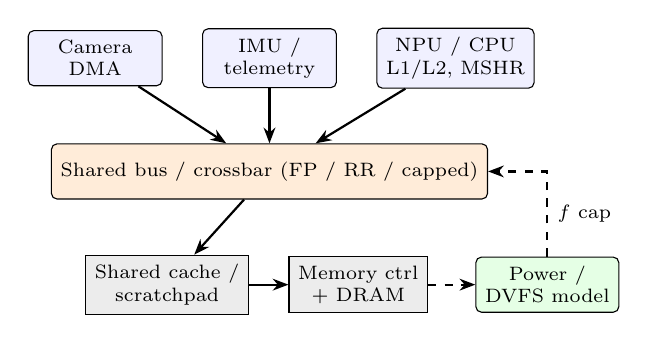
\begin{tikzpicture}[font=\scriptsize,node distance=5mm,
 blk/.style={draw,rounded corners=2pt,minimum height=7mm,minimum width=17mm,align=center,fill=blue!6},
 mem/.style={draw,minimum height=7mm,minimum width=17mm,align=center,fill=gray!15},
 ar/.style={-{Stealth[length=2mm]},thick}]
 \node[blk] (cam) {Camera\\DMA};
 \node[blk,right=of cam] (imu) {IMU /\\telemetry};
 \node[blk,right=of imu] (npu) {NPU / CPU\\L1/L2, MSHR};
 \node[blk,fill=orange!15,below=7mm of imu,minimum width=48mm] (bus) {Shared bus / crossbar (FP / RR / capped)};
 \node[mem,below=7mm of bus,xshift=-13mm] (llc) {Shared cache /\\scratchpad};
 \node[mem,right=of llc] (dram) {Memory ctrl\\+ DRAM};
 \node[blk,fill=green!10,right=6mm of dram,minimum width=17mm] (pw) {Power /\\DVFS model};
 \draw[ar] (cam)--(bus); \draw[ar] (imu)--(bus); \draw[ar] (npu)--(bus);
 \draw[ar] (bus)--(llc); \draw[ar] (llc)--(dram); \draw[ar,dashed] (dram)--(pw);
 \draw[ar,dashed] (pw.north) |- node[pos=0.25,right]{$f$ cap} (bus.east);
\end{tikzpicture}
\caption{Block diagram of the modelled SoC.}\end{figure}
\paragraph{Masters.} The camera DMA streams periodic frames at 30 or 60 fps (swept to 120) with configurable burst sizes of 64~B to 2~KB. The IMU/telemetry master emits small packets at 200--1000~Hz. The NPU/CPU reads tiles and writes features, with private L1/L2 caches and MSHRs.
\paragraph{Interconnect.} One shared bus or crossbar with three arbiters: fixed priority ($\imu>\npu>\cam$), round-robin, and bandwidth-regulated (burst-capped). The bus is non-preemptive.
\paragraph{Memory.} A shared cache or scratchpad (configurable size, associativity, write-back or write-through) in front of a memory controller and DRAM.
\paragraph{Power.} The power model tracks bus transfers, cache misses and compute activity, and lowers the clock to hold a power cap.

\section{Analytical Model}
\subsection{Utilisation and burst efficiency}
\begin{equation}
D_c=\phi F,\quad D_i=\lambda_i S_i,\quad \rho=\frac{D_c+D_i+D_n}{BW\,\eta(B)},\quad \eta(B)=\frac{B}{B+B_o}.
\end{equation}
\subsection{Blocking bounds}
\begin{align}
W^{\mathrm{FP}}_i&\le t_a+B_{\max}/BW,\\
W^{\mathrm{RR}}_i&\le t_a+(N-1)B_{\max}/BW,\\
W^{\mathrm{cap}}_i&\le t_a+B_{\mathrm{cap}}/BW.
\end{align}
Capping shortens blocking but lengthens the frame transfer, $T_c=\lceil F/B_{\mathrm{cap}}\rceil(B_{\mathrm{cap}}+B_o)/BW$, so the best cap balances IMU tail latency against frame time. The bounds ignore queueing and are written before any simulation so that they can be checked against it.
\subsection{Age, deadline slack and power}
\begin{align}
A_k&=t^{\mathrm{done}}_k-t^{\mathrm{cap}}_k,\qquad s_j=d_j-(t-t^{\mathrm{arr}}_j)-B_j/BW,\\
P&=P_s+\alpha CV^2f+e_b r_{\mathrm{DRAM}},\qquad f=\max\{f'\le f_{\max}:P(f')\le P_{\mathrm{cap}}\},\\
E&=\frac{1}{N_{\mathrm{proc}}}\int P\,dt .
\end{align}
\subsection{Equal-budget rule}
\begin{equation}
|\bar r^{\,\pi}_{\mathrm{DRAM}}-\bar r^{\,\mathrm{drop}}_{\mathrm{DRAM}}|\le\epsilon_b,\qquad |E^{\pi}-E^{\mathrm{drop}}|\le\epsilon_e .
\end{equation}
Frame dropping reaches a target budget by dropping a fraction $\delta$ of frames, $D_c\to(1-\delta)D_c$.

\section{Simulator and Trace Methodology}
\subsection{Event-driven core}
Time advances by discrete events: \texttt{IMU\_ARRIVAL}, \texttt{CAM\_FRAME\_START}, \texttt{DMA\_BURST\_REQ}, \texttt{BUS\_GRANT}, \texttt{CACHE\_HIT/MISS}, \texttt{DRAM\_SERVICE}, \texttt{COMPUTE\_TILE\_DONE}. Ties are broken by a fixed rule and all randomness uses seeded generators, so a run is reproducible.
\begin{algorithm}[h]\caption{Event loop with stall attribution}
\begin{algorithmic}[1]
\State push initial \texttt{IMU\_ARRIVAL}, \texttt{CAM\_FRAME\_START} events
\While{event queue not empty}
  \State $e \gets$ pop earliest event; $t \gets e.\mathrm{time}$
  \If{$e$ is a request arrival} \State enqueue at the arbiter; record $t^{\mathrm{arr}}$ \EndIf
  \If{bus free \textbf{and} arbiter has requests}
     \State $j \gets \textsc{Arbitrate}(\text{policy})$; split $j$ if policy requires
     \State charge $t-t_j^{\mathrm{arr}}$ to \emph{arbitration} or \emph{burst blocking}
     \State schedule \texttt{BUS\_GRANT} then cache lookup
  \EndIf
  \If{cache miss} \State charge \emph{cache}; if DRAM queue full charge \emph{DRAM saturation}; schedule \texttt{DRAM\_SERVICE} \EndIf
  \State update power model, possibly lower $f$ (Eq.\ for $f$)
\EndWhile
\end{algorithmic}\end{algorithm}
Arbitration wait is time spent behind requests of any class. Burst blocking is the part spent behind a burst that was already granted. Cache stalls come from conflict or capacity misses and MSHR exhaustion. DRAM saturation is time waiting for a full memory queue.
\subsection{Parameters}
\begin{table}[h]\centering\caption{Simulator parameters (defaults are assumed configuration values, fixed in the committed config file).}
\begin{tabular}{@{}lll@{}}\toprule Parameter & Default & Sweep\\\midrule
DRAM peak $BW$ & \tbd[12.8] GB/s & --\\
Row-hit / row-miss latency & \tbd[X] / \tbd[X] ns & --\\
Camera rate $\phi$ & 60 fps & 15--120\\
Frame size $F$ & \tbd[0.6] MB & \tbd[X]\\
Camera burst $B_c$ & 256 B & 64 B--2 KB\\
IMU rate / packet & 1 kHz / \tbd[32] B & 200--1000 Hz\\
Cache & \tbd[256 KB, 8-way, WB] & size, ways, WT/WB\\
MSHRs & \tbd[8] & 2--16\\
$P_s$, $\alpha C V^2$, $e_b$ & \tbd[X] & --\\
$P_{\mathrm{cap}}$, $f_{\max}$ & \tbd[X] W, \tbd[X] MHz & --\\
Queue limit $Q$ & \tbd[2] frames & 1--4\\
Seeds / clips & \tbd[N] & --\\\bottomrule\end{tabular}\end{table}
\subsection{Traces}
\textbf{Synthetic stress.} Sweep $\phi$, $F$, $B_c$ and background traffic to find the knee where $\rho=1$.\\
\textbf{Aerial.} For each ERA/CapERA clip~\cite{mou2020era,bashmal2023capera}, compute per-frame change intensity $m_k\in[0,1]$ (mean absolute difference between consecutive frames, optionally after registration). The NPU tile-read volume per frame scales with $m_k$, and frame arrival cadence follows the clip. IMU traffic is a logged or synthetic trace with bursts at manoeuvres. Clips are grouped by camera motion (still, moving, untrackable), as in~\cite{baig2026fewer}, and \tbd[N clips per group] are used.
\subsection{Validation}
Before reporting results: (i) conservation checks (bytes in equal bytes served), (ii) a single-master run matches $D/BW\eta$ within \tbd[X]\%, (iii) a two-master run matches Eqs.\ for $W^{\mathrm{FP}}$ and $W^{\mathrm{RR}}$, (iv) repeat runs with the same seed are bit-identical.

\section{Experimental Results and Ablations}
\subsection{Predicted against simulated}
\begin{table}[h]\centering\caption{Bound vs.\ simulated IMU wait at $B_c=1$~KB, 60 fps.}
\begin{tabular}{@{}lrrr@{}}\toprule Policy & Bound ($\mu$s) & Sim.\ \pone{} & Sim.\ max\\\midrule
Fixed priority&\tbd&\tbd&\tbd\\Round-robin&\tbd&\tbd&\tbd\\Burst-capped&\tbd&\tbd&\tbd\\\bottomrule\end{tabular}\end{table}
\subsection{H1: burst blocking}
\begin{figure}[h]\centering\begin{tikzpicture}\begin{axis}[dmaplot,xmode=log,log basis x=2,xlabel={Camera DMA burst $B_{c}$ (bytes)},
 ylabel={IMU \pone{} latency ($\mu$s)},xtick={64,128,256,512,1024,2048},xticklabels={64,128,256,512,1K,2K}]
\addplot table[col sep=comma,x=burst,y=fp]{data/burst.csv};\addlegendentry{Fixed prio.}
\addplot table[col sep=comma,x=burst,y=rr]{data/burst.csv};\addlegendentry{Round-robin}
\addplot table[col sep=comma,x=burst,y=cap]{data/burst.csv};\addlegendentry{Burst-capped}
\addplot table[col sep=comma,x=burst,y=adapt]{data/burst.csv};\addlegendentry{Adaptive split}
\end{axis}\end{tikzpicture}\illusnote
\caption{IMU \pone{} latency against camera burst size.}\end{figure}
\subsection{Saturation knee}
\begin{figure}[h]\centering\begin{tikzpicture}\begin{axis}[dmaplot,xlabel={Camera frame rate (fps)},ylabel={Utilisation $\rho$ / drop rate},
 ymin=0,ymax=1.05,legend style={at={(0.02,0.98)},anchor=north west}]
\addplot[blue,mark=*] table[col sep=comma,x=fps,y=rho]{data/knee.csv};\addlegendentry{$\rho$, power-capped}
\addplot[blue,dashed,mark=o] table[col sep=comma,x=fps,y=rho_pinned]{data/knee.csv};\addlegendentry{$\rho$, clock pinned}
\addplot[red,mark=square*] table[col sep=comma,x=fps,y=drop]{data/knee.csv};\addlegendentry{drop rate, power-capped}
\addplot[red,dashed,mark=square] table[col sep=comma,x=fps,y=drop_pinned]{data/knee.csv};\addlegendentry{drop rate, clock pinned}
\end{axis}\end{tikzpicture}\illusnote
\caption{Utilisation against frame rate; the knee is where $\rho=1$.}\end{figure}
\subsection{H2 and H3: equal-budget comparison}
\begin{figure}[h]\centering\begin{tikzpicture}\begin{axis}[dmaplot,xlabel={Frame drop rate (\%)},ylabel={Mean frame age at inference (ms)},
 legend style={at={(0.98,0.98)},anchor=north east}]
\addplot table[col sep=comma,x=drop,y=age]{data/policy_drop.csv};\addlegendentry{Frame dropping}
\addplot table[col sep=comma,x=drop,y=age]{data/policy_adapt.csv};\addlegendentry{Adaptive burst}
\addplot table[col sep=comma,x=drop,y=age]{data/policy_edf.csv};\addlegendentry{Age/deadline-aware}
\end{axis}\end{tikzpicture}\illusnote
\caption{Frame age against drop rate at equal bandwidth and energy.}\end{figure}
\begin{table}[h]\centering\caption{Equal-budget comparison (mean $\pm$ 95\% CI).}
\begin{tabular}{@{}lrrrrr@{}}\toprule Policy & IMU \pone{} & Max & Age (ms) & Drop (\%) & $E$ (mJ)\\\midrule
Frame dropping&\tbd&\tbd&\tbd&\tbd&\tbd\\Fixed burst, FP&\tbd&\tbd&\tbd&\tbd&\tbd\\Fixed burst, RR&\tbd&\tbd&\tbd&\tbd&\tbd\\
Burst-capped&\tbd&\tbd&\tbd&\tbd&\tbd\\Adaptive split&\tbd&\tbd&\tbd&\tbd&\tbd\\Age/deadline&\tbd&\tbd&\tbd&\tbd&\tbd\\\bottomrule\end{tabular}\end{table}
\subsection{Stall breakdown}
\begin{figure}[h]\centering\begin{tikzpicture}\begin{axis}[dmaplot,ybar stacked,bar width=11pt,ymin=0,ymax=100,ylabel={Share of stall cycles (\%)},
 symbolic x coords={FP,RR,Capped,Adaptive},xtick=data,legend style={at={(0.5,-0.18)},anchor=north,legend columns=2}]
\addplot[fill=blue!50] table[col sep=comma,x=policy,y=arb]{data/stall.csv};\addlegendentry{Arbitration wait}
\addplot[fill=orange!70] table[col sep=comma,x=policy,y=burst]{data/stall.csv};\addlegendentry{Burst blocking}
\addplot[fill=green!50!black] table[col sep=comma,x=policy,y=cache]{data/stall.csv};\addlegendentry{Cache miss}
\addplot[fill=gray!60] table[col sep=comma,x=policy,y=dram]{data/stall.csv};\addlegendentry{DRAM saturation}
\end{axis}\end{tikzpicture}\illusnote
\caption{Share of stall cycles by cause.}\end{figure}
\subsection{Energy and clocks}
\begin{figure}[h]\centering\begin{tikzpicture}\begin{axis}[dmaplot,xlabel={Policy},ylabel={Energy per processed frame (mJ)},
 ybar,bar width=12pt,symbolic x coords={Drop,FP,RR,Capped,Adaptive},xtick=data,ymin=0]
\addplot[fill=teal!50] table[col sep=comma,x=policy,y=energy]{data/energy.csv};
\end{axis}\end{tikzpicture}\illusnote
\caption{Energy per processed frame at equal bandwidth.}\end{figure}
\subsection{Ablations}
\begin{table}[h]\centering\caption{Planned ablations. Each changes one factor from the defaults.}
\begin{tabular}{@{}ll@{}}\toprule Factor & Values\\\midrule
Cache size / associativity & \tbd[X]\\Write policy & write-back vs.\ write-through\\MSHR count & 2, 4, 8, 16\\
Queue limit $Q$ & 1, 2, 3, 4\\Split size $B_s$ (adaptive) & 64 B, 128 B, 256 B\\Background traffic & off, 10\%, 30\%\\IMU rate & 200, 500, 1000 Hz\\\bottomrule\end{tabular}\end{table}
\tbd[Summarise which ablations change the ranking of policies.]

\section{Limitations and Threats to Validity}
\begin{itemize}
\item Simulator, not silicon: DRAM timing and power coefficients are modelled and assumed.
\item The latency bounds ignore queueing; agreement is tested, not assumed.
\item Aerial video sets traffic intensity only, not a real image pipeline.
\item The equal-budget tolerances $\epsilon_b,\epsilon_e$ are choices and the ranking may depend on them; report sensitivity.
\item Frame age is a proxy for task quality; \tbd[say whether motion-event recall was measured].
\end{itemize}

\section{Future Work}
Validate the simulator against a measured SoC or an FPGA bus model, add a priority-inversion study with a real flight-control loop, test learned arbiters against the age-aware rule, and extend to multi-camera setups.

\appendix
\section{Reproducibility}
\begin{itemize}
\item \texttt{sim/}: simulator source and config files; \texttt{traces/}: trace generators.
\item \texttt{results/}: raw CSV logs, one row per request with its stall cause.
\item \texttt{data/*.csv}: the aggregates read by the figures; set \verb|\illustrativefalse| in \texttt{common.tex} once they come from \texttt{results/}.
\item One script regenerates every table and figure from the committed logs.
\end{itemize}
\bibliographystyle{plain}
\bibliography{refs}
\end{document}
